\section{概述}

操作系统(Operating System)是控制应用程序执行的程序,并充当应用程序和计算机硬件之间的接口。它有下面三个目标:
\begin{itemize}
  \item 方便:操作系统是计算机更易于使用。
  \item 有效:操作系统允许以更有效的方式使用计算机系统资源。
  \item 扩展能力:在构造操作系统时,应该允许在不妨碍服务的前提下有效地开发、测试和引进新的系统功能。
\end{itemize}

作为用户/计算机接口下的操作系统,提供了程序开发、程序运行、输入输出设备访问、文件访问控制、系统访问、错误检测和相应。
作为资源管理器的操作系统,包括内核程序和当前正在使用的其他操作系统程序,统筹软硬件。
作为扩展机的操作系统,能够不断发展。

操作系统是最复杂的软件之一,这反映在为了达到那些困难的甚至相互冲突的目标而带来的挑战上。
操作系统开发中5个重要的理论\cite{denn80a}:
\begin{itemize}
  \item 进程
  \item 内存管理
  \item 信息保护和安全
  \item 调度和资源管理
  \item 系统结构
\end{itemize}

该操作系统实现了基本的进程管理、内存管理、窗口和图层管理,以及简陋的文件管理。

下面的截图展示了操作系统的实际运行效果。

\begin{figure}[htp]
    \centering
    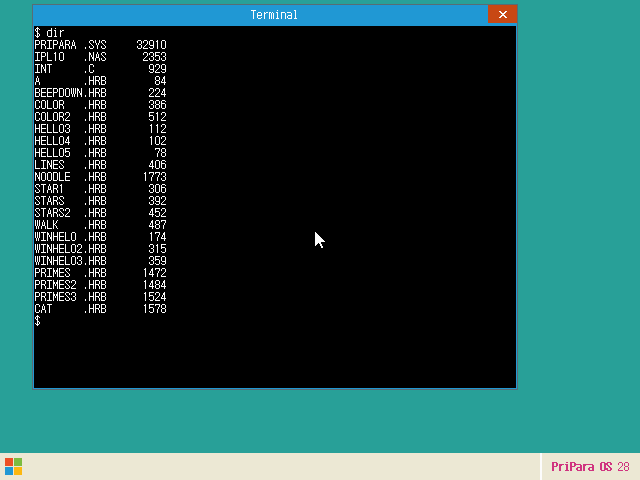
\includegraphics[width=12cm]{image/p1.png}
    \caption{}
    \label{fig:p1}
\end{figure}

% \begin{figure}[htp]
%     \centering
%     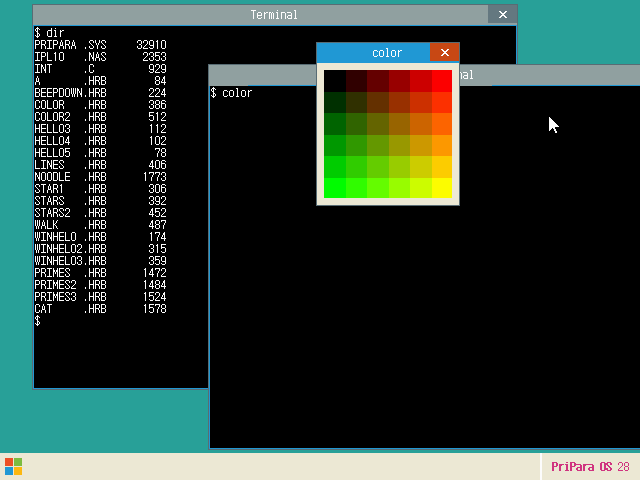
\includegraphics[width=12cm]{image/p2.png}
%     \caption{}
%     \label{fig:p2}
% \end{figure}

\begin{figure}[htp]
    \centering
    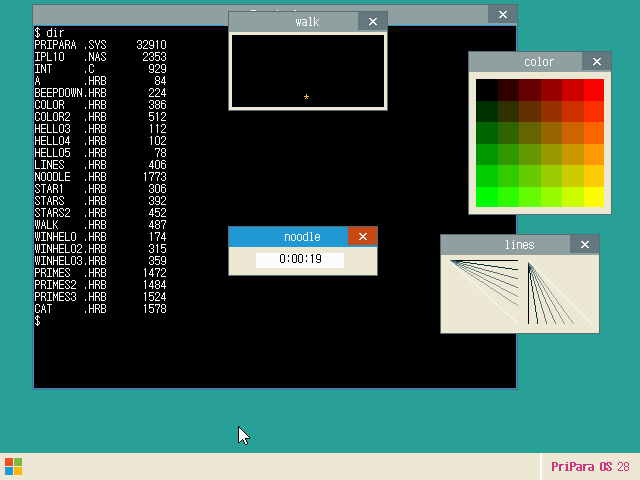
\includegraphics[width=12cm]{image/p3.png}
    \caption{}
    \label{fig:p3}
\end{figure}

\begin{figure}[htp]
    \centering
    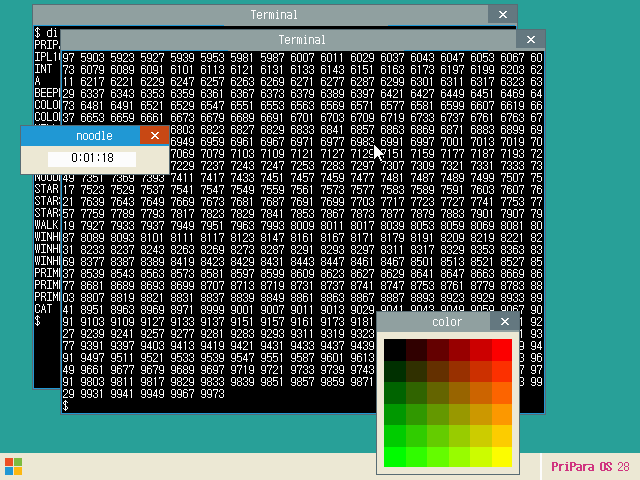
\includegraphics[width=12cm]{image/p4.png}
    \caption{}
    \label{fig:p4}
\end{figure}


%
% \subsection{进程}
%
% 进程(process),是计算机中已运行程序的实体。进程为曾经是分时系统的基本运作单位。
%
% 一个计算机系统进程包括下列数据:
% \begin{itemize}
%   \item 那个程序的可运行机器码的一个在存储器的映像。
%   \item 分配到的存储器。存储器的内容包括可运行代码、特定于进程的数据、调用堆栈、堆栈。
%   \item 分配给该进程的资源的操作系统描述符,诸如文件描述符、数据源和数据终端。
%   \item 安全特性,诸如进程拥有者和进程的权限集。
%   \item 处理器状态,诸如寄存器内容、物理存储器定址等。当进程正在运行时,状态通常存储在寄存器,其他情况在存储器。
% \end{itemize}
%
% 进程在运行时,状态(state)会改变。所谓状态,就是指进程目前的动作:
% \begin{itemize}
%   \item 创建(new):进程新产生中。
%   \item 运行(running):正在运行。
%   \item 等待(waiting):等待某事发生,例如等待用户输入完成。亦称“阻塞”(blocked)。
%   \item 就绪(ready):排班中,等待CPU。
%   \item 完成(finish):完成运行。
% \end{itemize}
%
% \subsection{存储器管理}
